% So we make this "beamer" rather than document!

\documentclass[11pt]{beamer}
% For handout add ,handout after 11pt

\usetheme[sectionpage=none,numbering=none]{metropolis}           % Use metropolis theme
	% To do printouts, add ", handout"  after aspectratio.
\usepackage{booktabs}
\usepackage{graphicx}
\usepackage{color}

\title{Welcome to Unifying Data Science!}
\author{\small Nick Eubank}
\date{\vspace*{.3in} \date}


% This is the beginning of a real document!
\begin{document}


\begin{frame}[c]
\maketitle
\end{frame}

\begin{frame}[c]{Three Goals of the Course}
By the end of this course, you will:
  \begin{enumerate}
    \pause \item Understanding how different approaches to data science relate to one another, and know when to employ different toolsets. \\
  \emph{The ``Unifying'' in Unifying Data Science}  
    \pause \item Be able to critically evaluate causal claims, and develop research designs to answer causal questions.  \\
  \emph{Causal Inference}
  \pause \item Execute a data science project from conception to delivery \\
  \emph{Complete with step-by-step models}
\end{enumerate}
\end{frame}



\begin{frame}[c]{}
  \centering 
  Part One: Unifying Data Science
\end{frame}

\begin{frame}[c]{How did Data Science become a thing?}

\begin{itemize}
    \pause \item Academic research is organized into silos:
    \pause
    \begin{itemize}
        \item Computer Science
        \item Statistics
        \item Economics
        \item Political Science
        \item Engineering
    \end{itemize}
\end{itemize}
\pause $\Rightarrow$ Development of new tools occurred \emph{within} each silo.
\end{frame}


\begin{frame}[c]{Where are we today?}
Very little cross-pollination across silos
\begin{itemize}
    \pause \item Lots of duplication of development.
    \pause \item Every silo has its own vocabulary.
    \pause \item Each silo has focused on the aspects most relevant to their applications. e.g.:
    \begin{itemize}
        \pause \item CS likes to classify things and make predictions, don't care how model works
        \item Social scientists like to make causal statements, don't care about predictive power
    \end{itemize}
\end{itemize}
\end{frame}

\begin{frame}[c]{Blind Men and the Elephant}
\pause 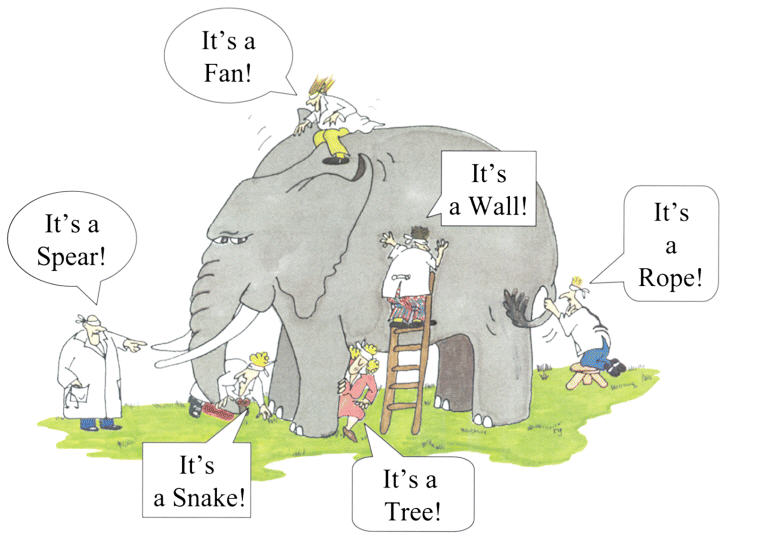
\includegraphics[width=\textwidth]{blindmenelephant.jpg}
\pause $\Rightarrow$ This is where data science is \emph{now.}
\end{frame}

\begin{frame}[c]{What do I think Data Science should be?}
\pause An effort to unify the development of quantitative methods \\
\pause $\rightarrow$ Recognize the elephant
\end{frame}

\begin{frame}[c]{This Class}
Discipline of learning how best to \alert{answer questions} using \alert{quantitative data.}
\end{frame}

\begin{frame}[c]{This Class}
\begin{enumerate}
  \item Introduce a taxonomy of questions \\
  {\color{gray} Exploratory, passive-predictive, causal}
  \pause \item \alert{For each class of questions}, we will discuss:
  \begin{itemize}
    \item Intrinsic challenges to answering each class of questions
    \item What tools are best suited to each type of question
  \end{itemize}
\end{enumerate}
  \pause   By the end of the course, you should know when to reach for...
  \begin{itemize}
    \pause \item Unsupervised machine learning
    \item Supervised machine learning
    \item Range of causal inference techniques
    \item Other approaches to exploratory analysis
  \end{itemize}
\end{frame}


\begin{frame}[c]{This Class}
The tool you use should be dictated by the question you seek to answer
\end{frame}


\begin{frame}[c]{Who Are We?}
  I am a empirical / computational social scientist
  \begin{itemize}
      \pause \item PhD in Political Economy, Masters in Economics, BA in Economics and International Relations
  \item Research on criminal justice, policing, social networks, election administration, gerrymandering, and (in days gone by) international development. 
  \end{itemize}
  \pause (But I have a pretty strong CS background for a social scientist.)\\
\vspace*{0.2cm}
\pause Erika Fox \& Clarissa Ache Cabello (TA) 
\begin{itemize}
  \pause \item MIDS Second Year Students
   \item \emph{Extremely} good at this
   \pause \item Causal inference is a discipline that people spend their careers studying, so they are terrific resources, but also be aware you may hit questions they redirect to me. 
\end{itemize}
\end{frame}


\begin{frame}[c]
  \centering
  Part Two: Causal Inference
\end{frame}

\begin{frame}[c]{Modeling and Representation of Data}
  \centering
       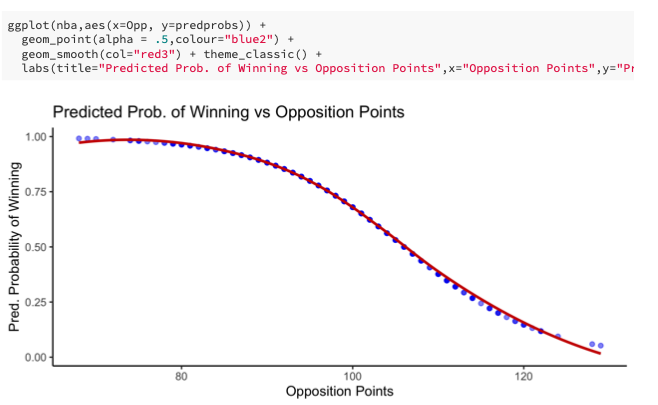
\includegraphics[width=0.5\textwidth]{logit.png} \\
       You learned a \emph{lot}:
       \begin{itemize}
          \item Model selection 
          \item Interpreting BIC, AIC, AUC, R-squared
          \item Residual Plots
       \end{itemize}
       \pause $\Rightarrow$ Develop model to \alert{faithfully represent patterns in the data}
\end{frame}


\begin{frame}[c]{Causal Inference}
  We're focused on what comes \alert{next}.\\
\pause \emph{Assume} our model faithfully represents the data. \\
\pause $\Rightarrow$ \alert{Given those models, what can we conclude \textbf{about the world}?} \\
\vspace*{0.3cm}
\pause Suppose we find a correlation between car advertising and consumer spending across neighborhoods in North Carolina.
\begin{itemize}
  \pause \item Does that imply that more advertising would increase spending further? \\
  \pause In other words, based on this model, do we think advertising is \emph{causing} more consumer spending?
\end{itemize}
\end{frame}

\begin{frame}[c]
  \frametitle{Causal Inference}
\centering
Correlation does not imply causation
\end{frame}

\begin{frame}[c]
  \centering
  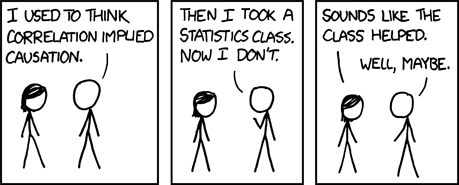
\includegraphics[width=\textwidth]{xkcd_correlation_causation.png}
\end{frame}

\begin{frame}[c]{Causal Inference}
Does advertising cause increased consumer spending?
  \begin{itemize}
  \pause \item ``Well, correlation does not imply causation, so I can't say.''
  \pause \item ``Well, correlation does not imply causation, \emph{but} yea probably.''
\end{itemize}
\end{frame}

\begin{frame}[c]{Causal Inference}
Correlation does not \emph{necessary} imply causation, 
\begin{itemize}
  \pause \item  but when certain assumptions are met, correlation \emph{does} imply causation. 
\end{itemize} 
\vspace*{0.2cm}
\pause By learning the \emph{assumptions} that are required for a correlation to be a good estimate of a causal effect, you can:
\begin{itemize}
  \pause \item Evaluate whether those assumptions are likely to be met,
  \pause \item Come up with different research designs whose assumptions \emph{would} be met. 
\end{itemize}
\end{frame}

\begin{frame}[c]
  \frametitle{Causal Inference}
  \centering
  \textbf{Modeling} \\
  Developing Model to Faithfully Represent Data \\
  \vspace*{1cm}
  $\Downarrow$ \\
  \vspace*{1cm}
   \alert<2->{\textbf{Inference}} \\
  \alert<2->{Interpreting Model Parameters}
\end{frame}

\begin{frame}[c]{Causal Inference}
While we will use a ``statistical framework'' (Potential Outcomes Framework) to help us be rigorous in our thinking... \\
\vspace*{0.2cm}
\pause There are \textbf{NO} statistical tests that will tell you if your model is estimating a true causal effect. \\
\begin{itemize}
  \pause \item \emph{Fundamental Problem of Causal Inference}
\end{itemize}
\vspace*{0.2cm}
\pause Causal inference is \alert{unavoidably} about: 
\begin{itemize}
  \item Critical thinking
  \item Case knowledge
\end{itemize}
\end{frame}

\begin{frame}[c]\frametitle{Causal Inference}
After introducting Potential Outcomes, we'll explore a range of causal research techniques:
\begin{itemize}
  \pause \item Experiments (Randomized-Control Trials, or RCTs)
  \pause \item Linear Regressions as Causal Tools 
  \pause \item Matching 
  \pause \item Differences in Differences
  \pause \item Natural Experiments
\end{itemize}
\pause $\Rightarrow$ Each of these designs will provide causal estimates \alert{if certain assumptions are met}, 
\begin{itemize}
  \pause \item But it will always be is up to you, the researcher, to evaluate whether those assumptions are reasonable!
\end{itemize}
\end{frame}

\begin{frame}[c]{Causal Inference}
  By the end of this course, you will:
  \begin{itemize}
      \item Understand why causal inference is hard, \\
      \pause \item Be able to critically evaluate causal evidence collected by others, \\
      \pause \item Articulate causal questions, \\
      \pause \item And develop research designs to answer those questions. 
  \end{itemize}
  \end{frame}
  

\begin{frame}[c]
  \centering
  Part Three: Your Data Science Project
\end{frame}

\begin{frame}[c]{Data Science Project}
Over semester, you will also develop a data science project from start-to-finish
\begin{itemize}
  \item Teams of 3-4,
  \item On topic of your own choosing.
  \item Only rule: it has to be causal.
\end{itemize}
\pause $\rightarrow$ Nice portfolio piece\\
\pause $\rightarrow$ MIDS first-years: Capstone with training wheels
\end{frame}


\begin{frame}[c]{Data Science Project}
  Introducing in stages:
  \begin{itemize}
    \pause \item Stakeholder management 
    \pause \item Backwards Design
    \pause \item Workflow Management 
    \pause \item Presenting to Different Audiences 
    \pause \item Giving Feedback
  \end{itemize}
\end{frame}
  


\begin{frame}[c]{Things to Know}
\begin{itemize}
\item Course site: \url{http://www.unifyingdatascience.org} \\
\alert{Contents subject to change!}
\pause \item Readings are \emph{incredibly} important. \\
\pause \item Reading reflections for every reading. \\
Due \textbf{7 am morning of class.} \\
\pause \item If you don't know git or github, you'll want to learn that early.
\begin{itemize}
\item Data Camp and Practical Data Science tools will be made available
\item Workshops hosted by Library
\end{itemize}
\end{itemize}
\end{frame}

\begin{frame}
\frametitle{If you have issues...}
\begin{itemize}
  \pause \item With the course material,
  \pause \item With the course design,
  \pause \item With learning online,
  \pause \item With the isolation associated with COVID-life,
  \pause \item \emph{Or anything else}...
\end{itemize}
\pause \textbf{Talk to me!}
\end{frame}

\begin{frame}[c]
\centering
Phew. That's it!   \\
Questions?
\end{frame}
\end{document}
